\documentclass[a4paper,11pt,onecolumn,twoside]{article}
\usepackage{ctex}
\usepackage{emptypage} 
\usepackage{fancyhdr}
\usepackage{amsmath,amsfonts,amssymb}
\usepackage{graphicx}
\usepackage{mathptmx}
\usepackage{booktabs}
\usepackage[labelfont=bf]{caption}
\usepackage{indentfirst}
\usepackage{caption}
\usepackage{enumitem}
\usepackage{subfigure}
\usepackage{fontspec}
\usepackage{xeCJK}
\usepackage[marginal]{footmisc}
\usepackage{subfigure}
\usepackage{fontspec}
\usepackage{setspace}
\usepackage{listings}
\usepackage{xcolor}
\usepackage{float}

% Please change the following fonts if they are not available.
\setmainfont{Times New Roman}
\setCJKmainfont[BoldFont=SimHei,ItalicFont=KaiTi]{SimSun}

\lstset{
	backgroundcolor=\color{green!10!blue!15},%代码块背景色
	rulesepcolor= \color{red!40!blue!100}, %代码块边框颜色
	breaklines=true,  %代码过长则换行
	breakatwhitespace=false,
	numbers=left, %行号在左侧显示
	numberstyle= \small,%行号字体
	keywordstyle= \color{blue},%关键字颜色
	commentstyle=\color{gray}, %注释颜色
	frame=shadowbox%用方框框住代码块
}


\addtolength{\topmargin}{-54pt}
%\setlength{\oddsidemargin}{-0.9cm}
%\setlength{\evensidemargin}{\oddsidemargin}
\setlength{\textwidth}{17.00cm}
\setlength{\textheight}{24.50cm}

\renewcommand{\baselinestretch}{1.1}
\parindent 22pt

\title{\textbf{[这是论文的标题]}}
\author{
[作者1姓名]\\[2pt]
{\small \textit{[南京大学XXXX学院2015级,南京 210046]}}\\[2pt]
 [作者2姓名]\\[2pt]
 {\small \textit{[南京大学XXXX学院2015级,南京 210046]}}\\[6pt]
指导老师:[指导老师1姓名]\\[2pt]
{\small \textit{[南京大学XXXXXX学院,南京 210046]}}\\[2pt]
指导老师:[指导老师2姓名]\\[2pt]
{\small \textit{[南京大学XXXXXX学院,南京 210046]}}\\[2pt]
}
\date{}


\pagestyle{fancy}
\fancyhf{}
\fancyhead[C]{南京大学第23届基础学科论坛 \\ The 23\textsuperscript{rd} Forum of Sciences and Arts}
\fancyhead[R]{[论文类别]}
\fancyhead[L]{[作者]}


\setlist{nolistsep}
\captionsetup{font=small}

\newcommand{\supercite}[1]{\textsuperscript{\cite{#1}}}
\begin{document}
\maketitle
\thispagestyle{fancy}
%\setlength{\oddsidemargin}{ 1cm}
%\setlength{\evensidemargin}{\oddsidemargin}
\setlength{\textwidth}{15.50cm}
\vspace{-.8cm}
\begin{center}
\parbox{\textwidth}{
\textbf{摘要} \quad {[\textbf{(方括号中的内容只是起到占位作用。请在使用模板时将它们(连同方括号本身)替换为论文的实际内容。)}这是样例文字。这是样例文字。这是样例文字。这是样例文字。这是样例文字。这是样例文字。这是样例文字。这是样例文字。这是样例文字。这是样例文字。这是样例文字。这是样例文字。这是样例文字。这是样例文字。这是样例文字。这是样例文字。这是样例文字。这是样例文字。这是样例文字。这是样例文字。这是样例文字。这是样例文字。这是样例文字。这是样例文字。这是样例文字。这是样例文字。这是样例文字。这是样例文字。这是样例文字。这是样例文字。这是样例文字。这是样例文字。]} \\

\textbf{关键词}\quad {[数学建模];[拉格朗日点];[国民经济]}}
\end{center}

\setcounter{page}{1}

\setlength{\oddsidemargin}{-.5cm}  % 3.17cm - 1 inch
\setlength{\evensidemargin}{\oddsidemargin}
\setlength{\textwidth}{17.00cm}

\section*{[引言]}
[这是样例文字。这是样例文字。这是样例文字。这是样例文字。这是样例文字。这是样例文字。这是样例文字。这是样例文字。这是样例文字。这是样例文字。这是样例文字。这是样例文字。这是样例文字。这是样例文字。这是样例文字。这是样例文字。这是样例文字。这是样例文字。这是样例文字。这是样例文字。这是样例文字。这是样例文字。这是样例文字。这是样例文字。这是样例文字。这是样例文字。这是样例文字。这是样例文字。这是样例文字。这是样例文字。这是样例文字。这是样例文字。这是样例文字。这是样例文字。这是样例文字。这是样例文字。这是样例文字。这是样例文字。这是样例文字。这是样例文字。这是样例文字。这是样例文字。这是样例文字。这是样例文字。这是样例文字。这是样例文字。这是样例文字。这是样例文字。这是样例文字。这是样例文字。这是样例文字。这是样例文字。这是样例文字。这是样例文字。]

[这是样例文字。这是样例文字。这是样例文字。这是样例文字。这是样例文字。这是样例文字。这是样例文字。这是样例文字。这是样例文字。这是样例文字。这是样例文字。这是样例文字。这是样例文字。这是样例文字。这是样例文字。这是样例文字。这是样例文字。这是样例文字。这是样例文字。这是样例文字。这是样例文字。这是样例文字。这是样例文字。这是样例文字。这是样例文字。这是样例文字。这是样例文字。这是样例文字。这是样例文字。这是样例文字。这是样例文字。这是样例文字。这是样例文字。这是样例文字。这是样例文字。这是样例文字。这是样例文字。这是样例文字。这是样例文字。这是样例文字。这是样例文字。这是样例文字。这是样例文字。这是样例文字。这是样例文字。这是样例文字。这是样例文字。这是样例文字。这是样例文字。这是样例文字。这是样例文字。这是样例文字。这是样例文字。这是样例文字。这是样例文字。这是样例文字。这是样例文字。这是样例文字。这是样例文字。这是样例文字。\footnote{这里是脚注。}]

[这是样例文字。这是样例文字。这是样例文字。这是样例文字。这是样例文字。这是样例文字。这是样例文字。这是样例文字。这是样例文字。这是样例文字。这是样例文字。这是样例文字。这是样例文字。这是样例文字。这是样例文字。这是样例文字。这是样例文字。这是样例文字。这是样例文字。这是样例文字。]

\section{[这是大标题]}
[这是样例文字。这是样例文字。这是样例文字。这是样例文字。这是样例文字。这是样例文字。这是样例文字。这是样例文字。这是样例文字。这是样例文字。这是样例文字。这是样例文字。这是样例文字。这是样例文字。这是样例文字。这是样例文字。这是样例文字。这是样例文字。这是样例文字。这是样例文字。这是样例文字。这是样例文字。这是样例文字。这是样例文字。这是样例文字。这是样例文字。这是样例文字。这是样例文字。这是样例文字。这是样例文字。这是样例文字。这是样例文字。这是样例文字。这是样例文字。这是样例文字。这是样例文字。这是样例文字。这是样例文字。这是样例文字。这是样例文字。这是样例文字。这是样例文字。这是样例文字。这是样例文字。这是样例文字。这是样例文字。这是样例文字。这是样例文字。这是样例文字。这是样例文字。这是样例文字。这是样例文字。]

\subsection{[这是小标题]}
[公式可以以行内或行间模式显示。 $\sum_{n = 1} ^ {\infty} 1/n^2 = \pi^2/6 $]

$$ \sum_{n=1}^{\infty} \frac{1}{n^2} = \frac{\pi^2}{6} $$

[如果你想给公式编号,请使用\texttt{equation}环境。]

  \begin{equation} \label{fourier}
    \mathcal{F}[f](\xi) = \int_{-\infty}^{\infty} f(x) e^{-2\pi ix \xi} dx
  \end{equation}

[这里是对上式的引用:式 \ref{fourier} 给出了$f$的傅里叶变换。]

  [另外,你也可以使用其他数学环境,例如 \texttt{split}, \texttt{align} 和 \texttt{gather}。]
  \begin{equation}
  \begin{split}
    (x+y)^4 &= (x+y)^2 (x+y)^2 \\
            &= (x^2+2xy+y^2)(x^2+2xy+y^2) \\
            &= x^4 + 4x^3y+6x^2y^2+4xy^3+y^4
  \end{split}
  \end{equation}

  \begin{align}
    \oint_S \mathbf{E} \cdot d \mathbf{s} &= \frac{Q}{\epsilon_0}
                                              \label{maxwell:begin} \\
    \oint_S \mathbf{B} \cdot d \mathbf{s} &= 0 \\
    \oint_L \mathbf{E} \cdot d \mathbf{l} &= -\frac{d\Phi_B}{dt} \\
    \oint_L \mathbf{B} \cdot d \mathbf{l} &= \mu_0 I +
               \mu_0 \epsilon_0 \frac{d\Phi_E}{dt} \label{maxwell:end}
  \end{align}
  [式 \ref{maxwell:begin} $\sim$ \ref{maxwell:end} 称为麦克斯韦方程组。]
  \begin{gather}
    (a + b)^2 = a^2 + 2ab + b^2      \notag   \\
    (a + b) \cdot (a - b) = a^2 - b^2
  \end{gather}


\subsection{[这里是小标题]}
[参考文献列表位于文档结尾的 \texttt{thebibliography} 环境中。如果要引用参考文献,请使用 \texttt{supercite} 命令。参考文献的编号会自动生成。例如:]

[这是样例文字。这是样例文字。这是样例文字\supercite{chendh, whiteside}。这是样例文字。这是样例文字。这是样例文字,\supercite{calms}这是样例文字。这是样例文字。这是样例文字。这是样例文字。这是样例文字。这是样例文字这是样例文字。这是样例文字。这是样例文字\supercite{obrien}。]

[你可以使用 \texttt{itemize} 或 \texttt{enumerate} 环境排版无序或有序列表。下面是一个无序列表:]
\begin{itemize}
    \item 这里是第一项;
    \item 这里是第二项;
    \item 这里是第三项。
\end{itemize}

[这是一个有序列表:]
\begin{enumerate}
    \item 这里是第一项;
    \item 这里是第二项;
    \item 这里是第三项。
\end{enumerate}

\subsection{[这是小标题]}
 [下面是一个图片的例子。]
\begin{figure}[H]
  \centering
  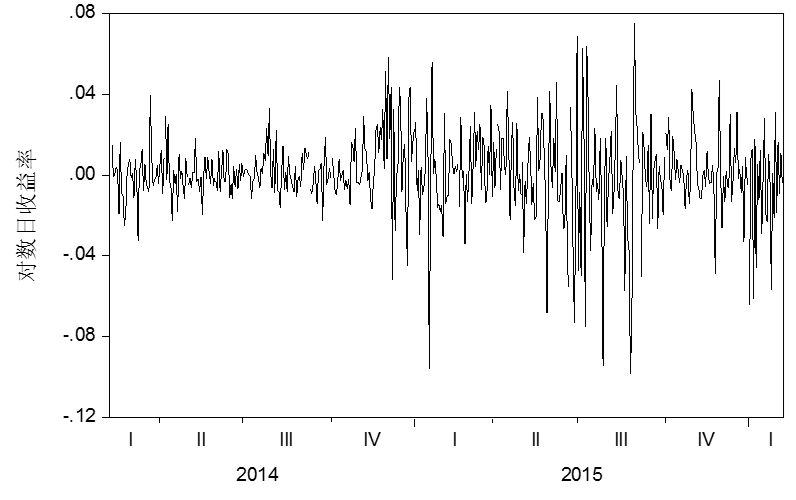
\includegraphics[width=0.7\textwidth]{figures/fig1.png}
  \caption{[这是一幅PNG图片]} \label{pngsample}
\end{figure}

[你也可以引用带标签的图片。例如:图\ref{pngsample}是一幅PNG图片。]

[你可以使用 \texttt{subfigure} 来排版子图,并且引用其中的某个特定子图。例如: 图 \ref{fig:subfig:d} 是第四幅子图。]
  \begin{figure}[H]
    \centering
    \subfigure[Sample 1]{
      \label{fig:subfig:a}
      
\includegraphics[width=3.5cm]{figures/sub1.png}}
    \hspace{1in}
    \subfigure[Sample 2]{
      \label{fig:subfig:b}
      
\includegraphics[width=3.5cm]{figures/sub2.png}}
    \hspace{1in} \\
    \subfigure[Sample 3]{
      \label{fig:subfig:c}
      
\includegraphics[width=3.5cm]{figures/sub3.png}}
    \hspace{1in}
    \subfigure[Sample 4]{
      \label{fig:subfig:d}
      
\includegraphics[width=3.5cm]{figures/sub4.png}}
    \caption{[这些都是子图。]}
    \label{fig:subfig}
  \end{figure}

\section{[这里是标题]}
[下面是表格的例子]
\begin{table}[H]
  \centering
  \begin{tabular}{ccccc}
    \midrule[1.5pt]
    A & B & C & D & E \\
    \hline
    1 & 0.165 & 0.165 & 13.401 & 0.000 \\
    2 & 0.254 & 0.233 & 45.243 & 0.000 \\
    3 & 0.228 & 0.171 & 71.021 & 0.000 \\
    4 & 0.150 & 0.054 & 82.226 & 0.000 \\
    5 & 0.117 & 0.009 & 89.015 & 0.000 \\
    6 & 0.106 & 0.016 & 94.599 & 0.000 \\
    7 & 0.124 & 0.059 & 102.34 & 0.000 \\
    8 & 0.077 & 0.011 & 105.30 & 0.000 \\
    9 & 0.079 & 0.010 & 108.41 & 0.000 \\
    10 & 0.092 & 0.033 & 112.70 & 0.000 \\
    11 & 0.050 & -0.006 & 113.96 & 0.000 \\
    12 & 0.096 & 0.048 & 118.60 & 0.000 \\
    \midrule[1.5pt]
  \end{tabular}
  \caption{[这是一张表格。推荐使用三线表。]}
\end{table}

\section{[结论]}
[这是样例文字。这是样例文字。这是样例文字。这是样例文字。这是样例文字。这是样例文字。这是样例文字。这是样例文字。这是样例文字。这是样例文字。这是样例文字。这是样例文字。这是样例文字。这是样例文字。这是样例文字。这是样例文字。这是样例文字。这是样例文字。这是样例文字。这是样例文字。这是样例文字。这是样例文字。这是样例文字。这是样例文字。这是样例文字。这是样例文字。这是样例文字。这是样例文字。这是样例文字。这是样例文字。这是样例文字。这是样例文字。这是样例文字。这是样例文字。这是样例文字。这是样例文字。这是样例文字。这是样例文字。这是样例文字。这是样例文字。这是样例文字。这是样例文字。这是样例文字。这是样例文字。这是样例文字。]

[这是样例文字。这是样例文字。这是样例文字。这是样例文字。这是样例文字。这是样例文字。这是样例文字。这是样例文字。这是样例文字。这是样例文字。这是样例文字。这是样例文字。这是样例文字。这是样例文字。这是样例文字。这是样例文字。这是样例文字。这是样例文字。]
					
%%%%%%%%%%%%%%%%%%%%%%%%%%%%%%%%%%%%%%%%%%%%%%%%%%%%%%%%%%%%%%%%
%  References
%%%%%%%%%%%%%%%%%%%%%%%%%%%%%%%%%%%%%%%%%%%%%%%%%%%%%%%%%%%%%%%%
\small
\begin{thebibliography}{99}
\setlength{\parskip}{0pt}
% There is no specific requirement on the format of references. You can follow the custom of your research field, and keep consistent throughout the paper.
\bibitem{chendh} 李晓寒,王宗笠,宁旭. 二维Ising模型临界相变的Monte-Carlo数值模拟.安徽大学学报(自然科学版),1000—2162 (2008) 03—0056—04: 56-59.
\bibitem{whiteside} 马文淦. 计算物理学. 北京: 科学出版社. 2005: 90-95.
\bibitem{calms} 梁淑英. 南京地区常见城市绿化树种的生理生态特性及净化大气能力的研究. 南
京林业大学硕士学位论文, 2005.
\bibitem{obrien} 张建军, 杨士普, 司江涛. 不同翼梢小翼对飞机横航向特性的影响. 飞行力学, 2011,
29(4): 1-1. % Book
\end{thebibliography}
\normalsize
\newpage

\begin{center}
{\Large \textbf{Effects of Dimension, Dispersion Relation and External Potential Field on the Thermodynamic Properties of Monoatomic Molecular Ideal Gas}} \\ [0.5cm]
{
Tingjun Zhang\\[2pt]
{\small \textit{2019, Kuang Yaming Honors School, Nanjing University, Nanjing 210046]}}\\[2pt]
Tingjun Zhang\\[2pt]
{\small \textit{2019, Kuang Yaming Honors School, Nanjing University, Nanjing 210046]}}\\[6pt]
Mentor: [Mentor Name]\\[2pt]
{\small \textit{[School of XXXXXXXXX, Nanjing University, Nanjing 210046]}}\\[2pt]
Mentor: [Mentor Name]\\[2pt]
{\small \textit{[School of XXXXXXXXX, Nanjing University, Nanjing 210046]}}\\[12pt]
}

\parbox{\textwidth}{
\textbf{Abstract:}\quad {In this paper, the influence of dimension, dispersion relationship (i.e., energymomentum
	relationship) and external potential field on the thermodynamic properties of monoatomic molecular
	ideal gas is discussed, in which only the harmonic oscillator potential is discussed as a sample of external potential
	field. For free particles (without external potential field), the density of particle states under different dimensions
	and dispersion relations is calculated first, then the partition function or the grand partition function is obtained, then
	the thermodynamic quantities are calculated, and the thermodynamic properties of the system are analyzed through
	the above results. For non-degenerate ideal gases which follow the Maxwell-Boltzmann distribution (which can
	also be considered as a system consisting of localized subsystems), the Maxwell speed distribution law in d dimensional
	space is also derived, and the main problems of kinetic theory of gases are discussed. For the case of external
	harmonic potential, the influence of dimension is mainly calculated.
	} \\

\textbf{Key words:}\quad {[Mathematical Modeling]; [Evaluation of Removal of Space Debris]; [Laser Generator]; [Satellit]}}
\end{center}

\end{document}
